\documentclass[12pt]{article}
\usepackage[english]{babel}
\usepackage{helvet}
%\usepackage[T1]{fontenc}
%\usepackage[latin9]{inputenc}
\usepackage[utf8]{inputenc}
\usepackage[a4paper]{geometry}
\geometry{verbose,tmargin=2.5cm,bmargin=2.5cm,lmargin=2.5cm,rmargin=2.5cm}
\setcounter{secnumdepth}{3}
\setcounter{tocdepth}{3}
\usepackage{color}
\usepackage{float}
\usepackage{amsmath}
\usepackage{amssymb}
\usepackage{graphicx}
\usepackage{setspace}
\usepackage{esint}
\usepackage{subfigure}
\usepackage{wrapfig}
\usepackage{cancel}
\usepackage{hyperref}


\title{Exercise Sheet 3}
\author{Uriel A. Aceves and Ana M. Montero}

\begin{document}
\maketitle

%\section*{IMPORTANTE}

%Probablemente ya estes dormido pero he pensado que igual mañana por la mañana de que te despiertes te apetece ponerte a hacer algo así que... :)

\section{Classical turning points}

In order to find the classical turning points we must be able to solve equation \ref{tp1} for $r$

\begin{equation}
    E = V(r).
    \label{tp1}
\end{equation}
For the hydrogen atom this equation looks like
\begin{equation}
    E = -\frac{Z}{r} + \frac{l(l+1)}{2r^2}.
    \label{tp2}
\end{equation}
We easily transform equation \ref{tp2} into a quadratic form
\begin{equation}
    Er^2 +Zr -  \frac{l(l+1)}{2} = 0,
\end{equation}
and use the quadratic formula to get $r$
\begin{equation}
    r\pm = \frac{-Z \pm \sqrt{Z^2 - 2El(l+1)}}{2E}.
    \label{tp3}
\end{equation}
Now it seems obvious that for every $l$ there will be two turning points.

We modified the previous programs kindly provided by Zhang Qian, and added the new features from this homework on top of the old ones. The definition of the array to store the turning points was made on the file \textit{orbit.py} on line 15 (Figure \ref{fig:tpdef}), and the calculations needed to obtain the turning points were made from line 37 to 39 (Figure \ref{fig:tpcalc})

\begin{figure}[h!]
    \centering
    
\includegraphics[width=\linewidth]{tp2}
    \caption{Definition of the array to store the turning points on file \textit{orbit.py}.}
    \label{fig:tpdef}
\end{figure}

\begin{figure}[h!]
    \centering
    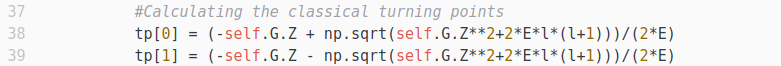
\includegraphics[width=\linewidth]{tp}
    \caption{Lines from file \textit{orbit.py} on which the calculation of the classical turning points occur.}
    \label{fig:tpcalc}
\end{figure}

\section{Normalize and estimate the contributions of the missing regions}

The normalization was already done in lines 74-75 of \textit{orbit.py} as shown in Figure \ref{fig:norm}

\begin{figure}[h!]
    \centering
    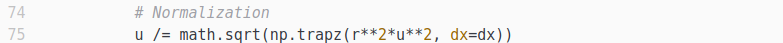
\includegraphics[width=\linewidth]{norm}
    \caption{Lines from file \textit{orbit.py} on which the calculation of the classical turning points occur.}
    \label{fig:norm}
\end{figure}

In section 2.6 of \cite{zhangQ} we can see more in detail how this formula arise.

The second part of the problem is to estimate the error we are making while integrating, due to the fact that we are not doing it from $-\infty$ to $\infty$ but from $x_{min}$ to $x_{max}$. An easy and reliable way to get such error is to approximate the tails of the functions with triangles. For instance, calculating the area of the triangle formed by the origin, the point $(x_{min},0)$ and $x_{min}, u(x_{min})$, the area of the triangle is then $u(x_{min})*x_{min}/2$. This solves just half of the problem, now we need to do the same for the part of the function we are neglecting on the right. For this case we will have two options: 1) The numerical value of the last component of $u$ on the array is numerically zero. 2) It is different than zero. On the former we don't need to perform any calculation, since the value of the integral of the right ``tail'' will be numerically zero. If the last component of $u$ in the array is not zero then we need to know how long (approximately) does the tail go until it reaches the value of zero (numerically) and then construct the triangle with the points $(x_{max},u(x_{max}))$, $(x_{max},0)$, $(x_{final},0)$, where $x_{final}$ is the first value of $x$ for which $u(x)$ is numerically zero. To know the value of the points while moving to the right of $x_{max}$ we use the asymptotic formulas. The implementation of this calculations is made on lines 83-91 of \textit{orbit.py} (Figure \ref{fig:norm2})   

\begin{figure}[h!]
    \centering
    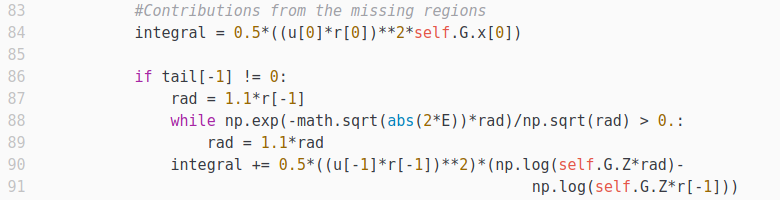
\includegraphics[width=\linewidth]{norm2}
    \caption{Lines from file \textit{orbit.py} on which the calculation of the missing contributions to the normalization integral is performed.}
    \label{fig:norm2}
\end{figure}

\section{Calculating $\Delta k_M^2$ to solve the eigenvalue problem}

So far the integration of the radial equation is performed correctly, but we have no way of knowing which are the correct energies given $n$, our strategy has been to make an initial guess and then start changing the energy until the forward and backward integration have the same logarithmic derivative at the matching point. This requires a lot of interaction with the user and it might be a slow process. With the purpose of making it more automated and less painful we will develop one way to choose automatically how do we need to change the value of the energy so that we get closer to the eigenenergy on every iteration.

Given an energy and a potential we can calculate the respective $k_i^2$ we use on the Numerov method (check equation 2.13 of \cite{zhangQ}). On the other hand, using equation 2.14 of \cite{zhangQ} we can solve for $k_i^2$ and obtain its value given $u$ and the computed values of $k_i^2$. If we do this we find

\begin{equation}
    k_i^2 = -\frac{6}{5\Delta x^2}\left[ \frac{\Tilde{u}_{i+1}\left(1+\frac{1}{12}\Delta x^2k_{i+1}^2\right) + \Tilde{u}_{i-1}\left(1+\frac{1}{12}\Delta x^2k_{i-1}^2\right)}{\Tilde{u}_i} -2\right].
    \label{k}
\end{equation}
This equation can be useful for us, specially when used in the matching point, that is $i=M$.

But there is also a $k_i^2$ calculated during the Numerov method implementation. The difference between both $k$ can hint at what the correction in the energy must be. Again using equation 2.13, we can obtain two different energies (depending on which k we use, the one used on the numerov method or the calculated using equation \ref{k} and the obtained values of $u$), if we take the difference of both equations we will find 

\begin{equation}
    \Delta E = \frac{1}{r_i}\left[\frac{\Delta k_i^2}{2} + r_i^2V(r_i) + \frac{1}{2}\left(l + \frac{1}{2}\right)^2\right].
    \label{deltE}
\end{equation}

The implementations of the here described calculations are in lines 77-81 (Figure \ref{deltk})

\begin{figure}[h!]
    \centering
    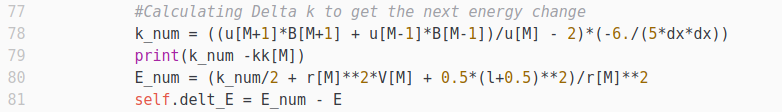
\includegraphics[width=\linewidth]{deltk}
    \caption{Lines from file \textit{orbit.py} on which the calculations depicted in equations \ref{k} and \ref{deltE} are performed.}
    \label{deltk}
\end{figure}
It was decided to make $\Delta E$ an attribute of the orbit class and therefore is defined as such in line 16 (Figure \ref{fig:delte}). The idea behind this was to be able to retrieve the computed energy change for the next step while doing the shooting method automatically.

\begin{figure}[h!]
    \centering
    
\includegraphics[width=\linewidth]{delte}
    \caption{Definition of the attribute \textit{delt\_E} on the file \textit{orbit.py}.}
    \label{fig:delte}
\end{figure}


\section{Using first order perturbation theory to change the energy}

Now we have a $\Delta E$ that we can use to automatize the shooting process. For this it would be helpful to remember how energies are modified in first order perturbation theory

\begin{equation*}
    E = E_0 + \lambda \Delta E,
\end{equation*}
in particular for us this equation would look like
\begin{equation}
    E_{new} = E_{old} + \lambda \Delta E,
    \label{newE}
\end{equation}
Let's remember that $\lambda$ is supposed to be a small value. A value of $\lambda$ that rendered good results is $\lambda = 1\times 10^{-4}$. The lines implementing equation \ref{newE} are 19 and 24 in Figure \ref{shoot}


\section{Initializing the wavefunctions}

The initial value we had previously are really good, since they depict the asymptotic behaviour, as shown in Table 2.3 of \cite{zhangQ}. Therefore we decided not to modify this particular lines of code. The implementations of the selection of the initial points are shown in Figure \ref{init}.

\begin{figure}[h!]
    \centering
    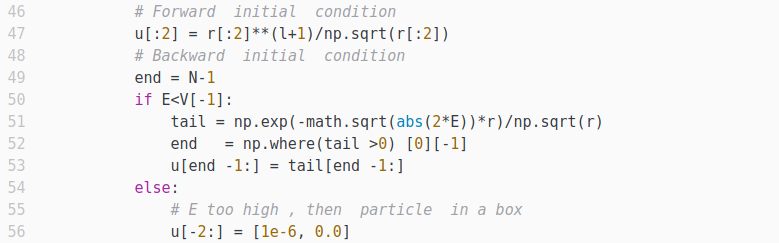
\includegraphics[width=\linewidth]{init}
    \caption{Initial values for the forward and backward integration in \textit{orbit.py}.}
    \label{init}
\end{figure}

\clearpage
\section{Stopping criteria}

We are almost ready. We have the initial values set, and we can compute from our initial guess, what the energy change should be for the next step. Now the idea is to automatize this process, i.e. we need to program an algorithm such that it performs the shooting calculations, obtains the $\Delta E$ to plug in the next shooting iteration and get closer to the desired eigenenergy, and repeats. Finally, we need criteria to know when to stop our search. For this matter, we can set an $\epsilon$ such that, when the difference in energy $\Delta E$ is smaller than this $\epsilon$ we can stop. 

It is important to notice that it is possible to have undesired situations, for example, we might start with a very high energy and while doing the iterations the program might get stuck around a false eigenenergy. These energies are solutions to the problem, but with a different number of nodes. So we need a mechanism to avoid getting stuck in those regions and to enable the program to escape from them. Hence, if the difference in energies from consecutive steps is smaller than our $\epsilon$ but we still don't have the desired number of nodes, we ``kick'' the energy a little bit so the program escapes the region and keeps looking for the correct eigenenergy. This ``kick'' is implemented in lines 25-26 of \textit{main.py} (Figure \ref{shoot}). The rest of the here described algorithm for searching eigenenergies is shown in the same figure.

\begin{figure}[h!]
    \centering
    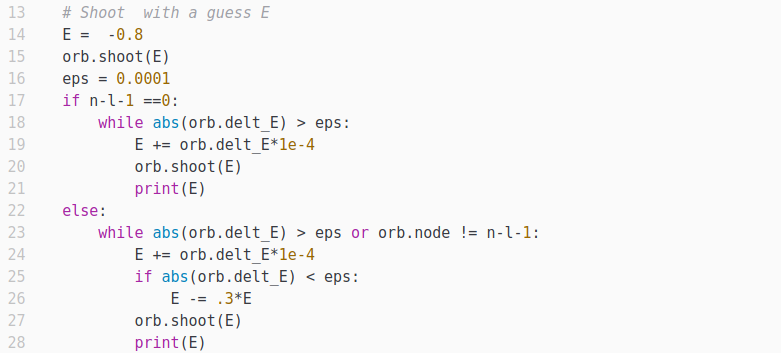
\includegraphics[width=\linewidth]{shoot}
    \caption{Implementation of the algorithm to update the energy until it converges to the desired value in \textit{main.py}.}
    \label{shoot}
\end{figure}

Finally we can see our tremendous success portrayed in Figure \ref{results}.

\begin{figure}
    \centering
    \subfigure[$u_{1,l}$]{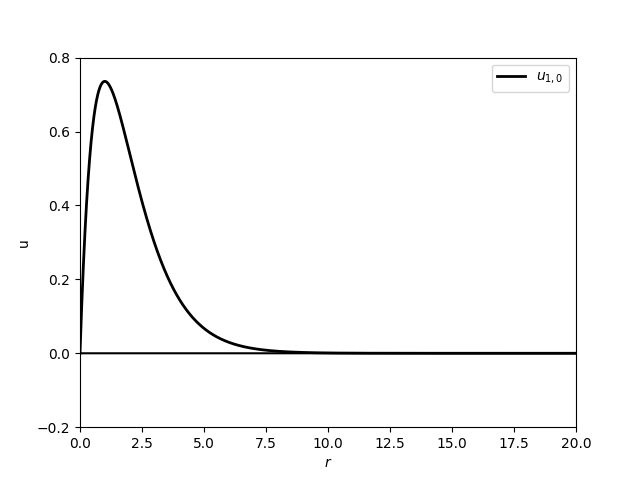
\includegraphics[height = 5.5cm]{u1.png}}
    \subfigure[$u_{2,l}$]{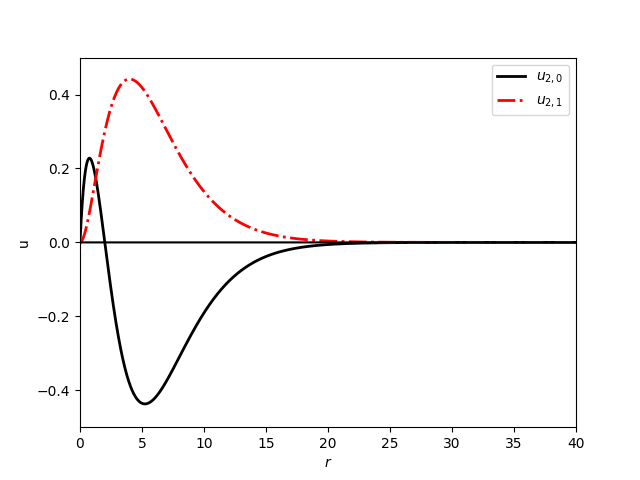
\includegraphics[height = 5.5cm]{u2.png}}
    \subfigure[$u_{3,l}$]{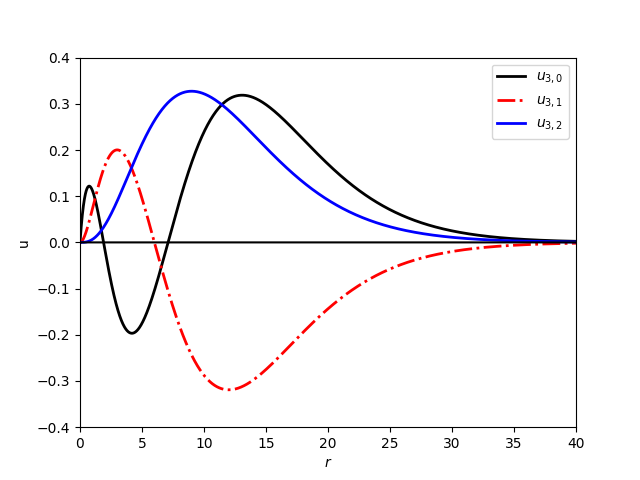
\includegraphics[height = 5.5cm]{u3.png}}
    \subfigure[$u_{4,l}$]{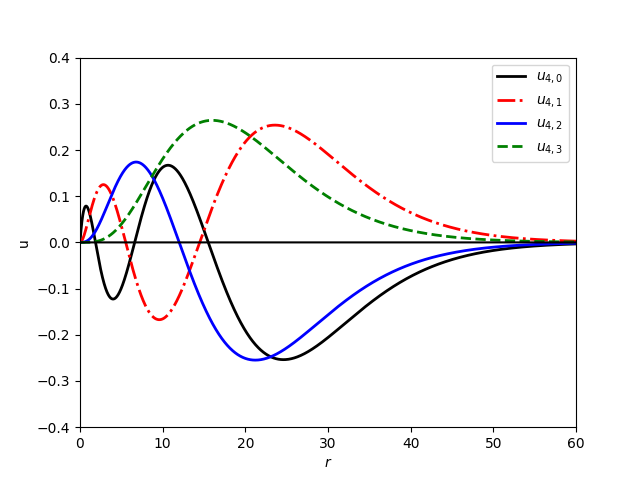
\includegraphics[height = 5.5cm]{u4.png}}
    \subfigure[$u_{5,l}$]{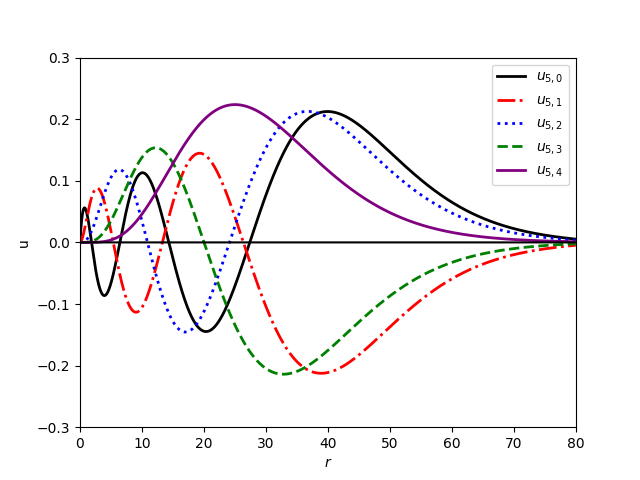
\includegraphics[height = 5.5cm]{u5.png}}
    \subfigure[$u_{6,l}$]{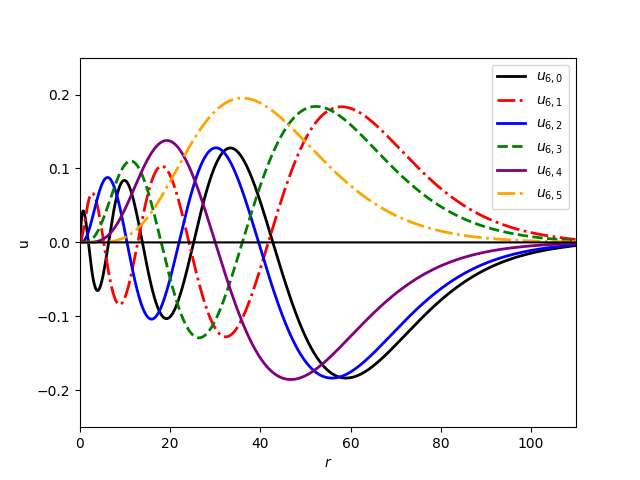
\includegraphics[height = 5.5cm]{u6.png}}
    \caption{Plots of the hydrogen radial wavefunctions for several values of $n$}\label{results}
\end{figure}

\begin{thebibliography}{9}% 2nd arg is the width of the widest label.
\bibitem{zhangQ} Zhang, Q. (September 2014). Calculations of atomic multiplets across the periodic table (Master’s thesis). Retrieved from https://juser.fz-juelich.de/record/188242/files/FZJ-2015-01684.pdf.
\end{thebibliography}

\end{document}